%
% This work is licensed under a Creative Commons Attribution-ShareAlike 4.0 International License.
%

\documentclass[10pt, a5paper, twoside, openany]{memoir}

\setsecnumdepth{subsection}

\title{Introduction to Quantum Mechanics}
\author{Joseph D. MacMillan}
\date{}


\usepackage{graphicx}
\usepackage{color} 
\usepackage{amsmath, amssymb}
\usepackage{libertinus}
\usepackage{microtype}
\usepackage{layout}
\usepackage[most]{tcolorbox}
\tcbuselibrary{skins,breakable}
\usepackage[hang, small, bf]{caption}
\captionsetup[table]{position=top}
\captionsetup[figure]{position=bottom}
\usepackage[hyphens]{url}
\usepackage[hidelinks]{hyperref}
\hypersetup{pdftitle={Introduction to Quantum Mechanics}}
\hypersetup{pdfauthor={Joseph D. MacMillan}}
\urlstyle{rm}


% Set page margins, etc
\setstocksize{9in}{6in}
\settrimmedsize{\stockheight}{\stockwidth}{*}
\settrims{0pt}{0pt}

\setlxvchars %define lenght 65 char of the used font
\settypeblocksize{*}{1.05\lxvchars}{1.7}
\setbinding{20pt} 
\setlength{\headheight}{30pt}
\setlength{\footskip}{20pt}

\setulmargins{90pt}{*}{*}
\setlrmargins{*}{*}{*}
\setheaderspaces{*}{30pt}{*}

\setmarginnotes{0.01pt}{20pt}{\onelineskip}
\checkandfixthelayout

\setcounter{tocdepth}{3}



\newcommand{\uu}{\symbfup{u}}
\newcommand{\grad}{\symbfup{\nabla}}
\newcommand{\curl}{\symbfup{\nabla} \times}
\newcommand{\dfdx}[2]{\frac{\partial {#1}}{\partial {#2}}}
\newcommand{\ddfdx}[2]{\frac{\partial^2 {#1}}{\partial {#2}^2}}
\newcommand{\vort}{\symbfup{\omega}}
\renewcommand\vec{\symbfup}
\newcommand{\unit}[1]{\hat{\vec{#1}}}
\newcommand{\U}{\mathbb{U}}
\newcommand{\V}{\mathbb{V}}
\newcommand{\LL}{\mathbb{L}^2}
\newcommand{\LLLL}{\mathbb{L}^4}

\newcommand{\ket}[1]{| #1 \rangle}
\newcommand{\bra}[1]{\langle #1 |}
\newcommand{\braket}[2]{\langle #1 | #2 \rangle}


%\DeclareMathAlphabet{\mathbfsf}{\encodingdefault}{\sfdefault}{bx}{sl}
\newcommand{\tens}[1]{\mathbfsfit{#1}}


\newcounter{example}[chapter]
\def\theexample{\thechapter.\arabic{example}}
\newenvironment{example}[1][ ]{\refstepcounter{example}
\begin{tcolorbox}[breakable, sharp corners, boxrule = 0pt, frame empty, opacityframe=0, parbox=false]
\textbf{Example \theexample \ -- #1.}
}
{ 
\end{tcolorbox}
}

\newenvironment{theorem}[1][ ]{
\begin{tcolorbox}[breakable, sharp corners, boxrule = 0pt, frame empty, opacityframe=0, parbox=false]
\textbf{#1.}
}
{ 
\end{tcolorbox}
}

\newcounter{problem}[chapter]
\def\theproblem{\thechapter.\arabic{problem}}
\newenvironment{problem}[1][ ]{\refstepcounter{problem} \noindent \textbf{Problem \theproblem \ -- #1.}}{\vspace{0.1in}}


\begin{document}

\frontmatter

\maketitle

\begin{center}


\includegraphics[width=\linewidth]{Figures/fig_cover_wave}

\vspace{1in}

{\small

This version was compiled on \today.  For the most up-to-date version and supplementary material, see \href{https://josephmacmillan.github.io/IntroductionToQuantumMechanics/index.html}{josephmacmillan.github.io/IntroductionToQuantumMechanics}.

\vspace{2in}

This work is licensed under a \href{https://creativecommons.org/licenses/by-sa/4.0/}{Creative Commons Attribution-ShareAlike 4.0 International License}.
}
\end{center}


\newpage

\tableofcontents

\chapter{Preface}

To come. 

\section{Why Open Education?}

This book and the supplementary material are released under a Creative Commons Attribution-ShareAlike 4.0 International License, which means you can do anything you want with this book:  cut out stuff you don't need, use it to build an even better book, download it for free off the web, print it out yourself, give it to your friends (they want a copy, trust me), and anything else you can think of.  The only stipulation is that you give credit where it's due, and release the derivative work under the same license.

Why did I choose this?  Because I've taught university courses and have seen the issues with expensive textbooks: students not being able to afford them, students finding illegal PDF copies online and sharing them, the publishing companies fighting back with various schemes like renting digital copes, and so on.  Especially in advanced physics, little textbooks can be so expensive, and yet I think textbooks are an important and necessary resource, and I want my students to all have a copy.

\section{Thanks}

To come.

\vspace{1in}

Find a typo, mistake, or horrible misconception in this book?  Let me know by creating a new issue at the GitHub page:  

\href{https://github.com/josephmacmillan/IntroductionToQuatumMechanics/issues}{github.com/josephmacmillan/IntroductionToQuantumMechanics/issues}.



\mainmatter

\chapter{The Stern-Gerlach Experiment}

\section{Spin Angular Momentum}

Let's start with a system that is pretty much as far away from the quantum world as possible -- the Earth and Sun, as shown in Figure \ref{fig_sun_earth}.  With its total motion, the Earth has two kinds of angular momentum:  \emph{orbital} angular momentum $\vec{L}$ from its orbit around the sun, and \emph{spin} angular momentum $\vec{S}$, resulting from its 24 hour rotation.  Of course, the spin angular momentum in this case is due to adding up the orbital angular momentum $\vec{L}_i = \vec{r}_i \times \vec{p}_i$ of each of the tiny pieces of the Earth, but we'll keep the distinction because this is definitively not the case in quantum systems as we'll see.  Note that the two kinds of angular momentum for the Earth point in different directions since the rotation axis of the Earth is tilted 23$^\circ$ from the orbital plane.

\begin{figure}
\centering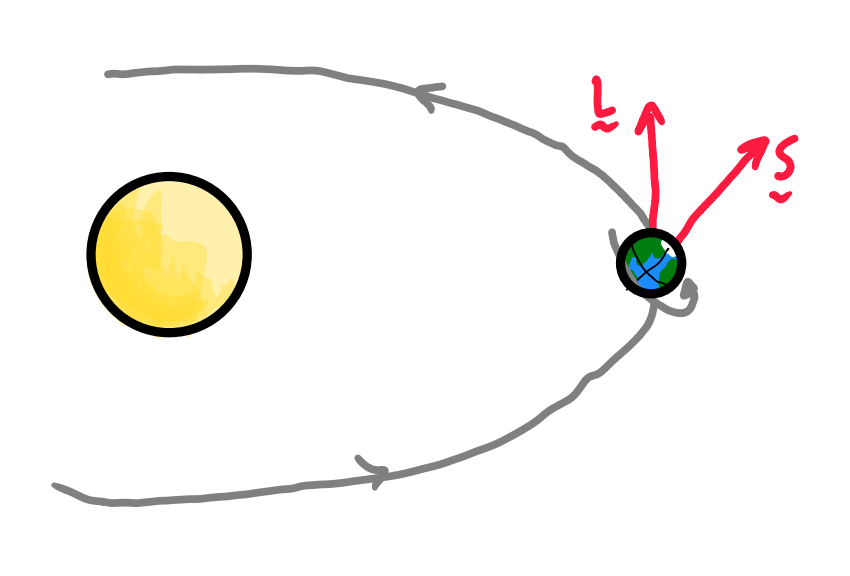
\includegraphics[width=0.5\linewidth]{Figures/Chapter 1/fig_sun_earth.png}
\caption{The Earth goes around the Sun every 365 days (orbital angular momentum) and rotates around its axis every 24 hours (spin angular momentum).}
\label{fig_sun_earth}
\end{figure}

As a simple quantum system, consider an electron in orbit around a proton -- a hydrogen atom.  The electron has orbital angular momentum just like the Earth (depending on what state it's in), and it also has spin angular momentum.  Careful, though, as the electron doesn't rotate like the Earth -- how can it when it has essentially no size or diameter to spin?  Despite this, it has measurable intrinsic angular momentum, which we'll call \emph{spin} $\vec{S}$.  Since spin is a vector, it has components $(S_x, S_y, S_z)$, and thus to specific the spin of the electron we use three different numbers; keep this in mind for later.

Suppose we put a stationary electron in a magnetic field $\vec{B}$.  Since the electron is stationary, the Lorentz force
\[
\vec{F} = q\vec{v} \times \vec{B}
\]
is zero.  But the electron's spin angular momentum gives it a magnetic dipole moment $\vec{\mu}$, and it's then possible for an \emph{inhomogeneous} magnetic field to exert a force (see Griffiths \emph{Introduction to Electrodynamics}, fourth edition, section 6.2)
\begin{equation}
\vec{F} = \grad (\vec{\mu} \cdot \vec{B}).
\end{equation}



%
%
%

\section{The Stern-Gerlach Experiment}

The 

%
%
%

\section{Extending the Experiments}

The 

%
%
%



\section*{Problems}
\addcontentsline{toc}{section}{Problems}
\markright{Problems}%

\begin{problem}[Electron spin]
How fast would the surface of an electron be going if it had ....
\end{problem}




\end{document}
